\documentclass{beamer} % Gliederung im Kopf, sections und subsections
\setbeamertemplate{navigation symbols}{}%remove navigation symbols

% \usepackage{tikz}
% \usetikzlibrary{shapes,arrows,positioning,chains,fit,calc,matrix,decorations.pathreplacing}
% \usepackage{xcolor}
% \usetikzlibrary{intersections}


\usepackage{tikz}
\usetikzlibrary{arrows,decorations.pathmorphing,backgrounds,positioning,fit,petri}
% \renewcommand*{\familydefault}{\sfdefault}

% \tikzset{forestyle/.style = {rectangle, thick, minimum width = 5cm, minimum height = 0.5cm, text width = 4.5cm, outer sep = 1mm},
%   pre/.style={<-, shorten <=1pt, >=stealth, ultra thick},
%   extend/.style={<-,dashed, shorten <=1pt, >=stealth, ultra thick}}



% \def\firstcircle{[name path=firstcircle] (0,0) circle (3cm)}
% \def\secondcircle{[name path=secondcircle] (55:3.11111cm) circle (3cm)} %No idea how the numbers selected work; they were derived from what I found online. They seem to function though!
% \def\thirdcircle{[name path=thirdcircle] (0:3.5cm) circle (3cm)}


\mode<presentation>

\begin{document}

\begin{frame}

    \begin{figure}[tb]
        \centering

        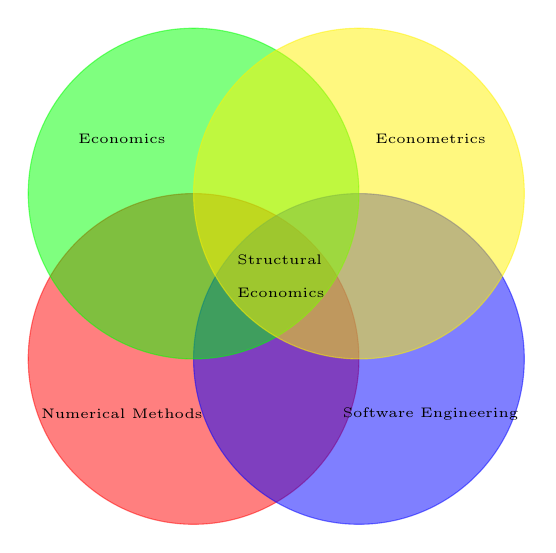
\begin{tikzpicture}[scale=.7]  % Use scale to change the figure's size

            % Circles
            \draw[red, fill=red, opacity=0.5] (0, 0) circle (3);
            \draw[blue, fill=blue, opacity=0.5] (3, 0) circle (3);
            \draw[green, fill=green, opacity=0.5] (0, 3) circle (3);
            \draw[yellow, fill=yellow, opacity=0.5] (3, 3) circle (3);

            % Text
            \draw (-1.3, -1) node {\tiny Numerical Methods};
            \draw (4.3, -1) node {\tiny Software Engineering};
            \draw (-1.3, 4) node {\tiny Economics};
            \draw (4.3, 4) node {\tiny Econometrics};

            \draw (1.8, 1.5) node[text width=40pt] {\tiny Structural Economics};

        \end{tikzpicture}

        \caption{Venn Diagram}
        \label{fig:venn_diagram}

    \end{figure}

\end{frame}
% \begin{frame}\begin{center}\begin{tikzpicture}
%     \begin{scope}[fill opacity=.5, text opacity=1]
%     \fill[red] \firstcircle;
%     \fill[green]\secondcircle;
%     \fill[blue]\thirdcircle;
%     \draw \firstcircle node[anchor=north west,name=A] {};
%     \draw \secondcircle node [above,name=B] {};
%     \draw \thirdcircle node [below,name=C] {};
%     \node at (25,1.75cm) {Structural Econometrics}
%     % \node at ($0.4*(B)+0.3*(C)+0.3*(A)$) {Structural};
%     % \node at ($0.25*(B)+0.375*(C)+0.375*(A)$) {Econometrics};
%     \path (-1cm,-1cm) node {Programmer}
%     (1.75cm,3.5cm) node {Economist}
%     (4.5cm,-1cm) node {Econometrician};
%     \end{scope}
% \end{tikzpicture}\end{center}\end{frame}


\end{document}
